%%%%%%%%%%%%%%%%%%%%%%%%%%%%%%%%%%%%%%%%%%%%%%%%%%%%%%%%%%%%%%%%%%%%%%%%
% Plantilla TFG/TFM
% Escuela Politécnica Superior de la Universidad de Alicante
% Realizado por: Jose Manuel Requena Plens
% Contacto: info@jmrplens.com / Telegram:@jmrplens
%%%%%%%%%%%%%%%%%%%%%%%%%%%%%%%%%%%%%%%%%%%%%%%%%%%%%%%%%%%%%%%%%%%%%%%%

\chapter{Estado del Arte}
\label{marcoteorico}

Antes de profundizar en los detalles técnicos, es importante estudiar contexto actual en el dominio de los buscadores multimedia basados en lenguaje natural. Este estudio permitirá asentar una fundamentación teórica y metodológica sólida, comprender los desafíos y las limitaciones identificadas en investigaciones previas e identificar las brechas en el conocimiento existente, así como las oportunidades para realizar contribuciones significativas en LLMSearch.

\section{Modelos de Lenguaje Natural (LLMs) para Búsqueda}

Los \textbf{\glspl{llm}} han revolucionado el procesamiento del lenguaje natural en los últimos años. Modelos como \emph{GPT-3} y \emph{GPT-4} demuestran que, con miles de millones de parámetros entrenados en enormes corpus de texto es posible comprender y generar lenguaje con notable fluidez y contexto. Estos modelos capturan representaciones semánticas ricas, lo que habilita nuevas maneras de buscar semanticamente y recuperar información.

\textbf{Características clave:}

\begin{itemize}
  \item \textbf{Búsqueda por significado}: En lugar de limitarse a coincidencias de palabras clave, un \gls{llm} puede interpretar la intención de una consulta en lenguaje natural y relacionarla con documentos relevantes aunque no compartan palabras literalmente.
  
  \item \textbf{Embeddings semánticos}: Técnicas como \emph{embeddings} de oraciones usando modelos tipo \gls{bert} o Sentence Transformers convierten documentos y consultas a vectores en un espacio vectorial común, donde la similitud de coseno permite recuperar los contenidos más cercanos en significado.
  
  \item \textbf{\gls{rag}}: Los \glspl{llm} pueden integrarse en pipelines donde primero se recuperan documentos candidatos y luego el modelo genera una respuesta o resumen usando esos textos.
  
  \item \textbf{Interfaz conversacional}: Modelos tipo ChatGPT permiten refinar iterativamente las consultas de búsqueda mediante diálogo, mejorando la precisión de resultados en consultas ambiguas.
\end{itemize}

Los avances más recientes se centran en mejorar la \textbf{eficiencia y apertura} de estos modelos. Mientras GPT-4 (de OpenAI) es de uso cerrado y con un tamaño muy grande no divulgado (>100B parámetros), han emergido modelos de código abierto como \emph{LLaMA} (Meta) y sus variantes, que con 7--70B parámetros logran desempeños competitivos.

\section{Modelos Visión-Lenguaje para Imágenes}

En un buscador multimedia, es esencial manejar consultas sobre contenido visual (imágenes) usando lenguaje natural. Aquí destacan los \textbf{modelos visiolingüísticos} o \textbf{\glspl{vlm}}, que conectan representaciones de imágenes con representaciones textuales en un espacio común.

\subsection{CLIP y Embeddings Multimodales}

Un hito fue el modelo \textbf{\gls{clip}} de OpenAI, que entrena conjuntamente un codificador de texto (transformer) y un codificador visual (Red Neuronal Convolucional o \gls{vit}) para proyectar ambos tipos de entrada en \textbf{vectores de embedding} de la misma dimensión. Mediante aprendizaje contrastivo en 400 millones de pares imagen--texto, \gls{clip} logró que textos e imágenes con contenido semántico equivalente quedaran cercanos en el espacio vectorial.

\begin{figure}[h]
  \centering
  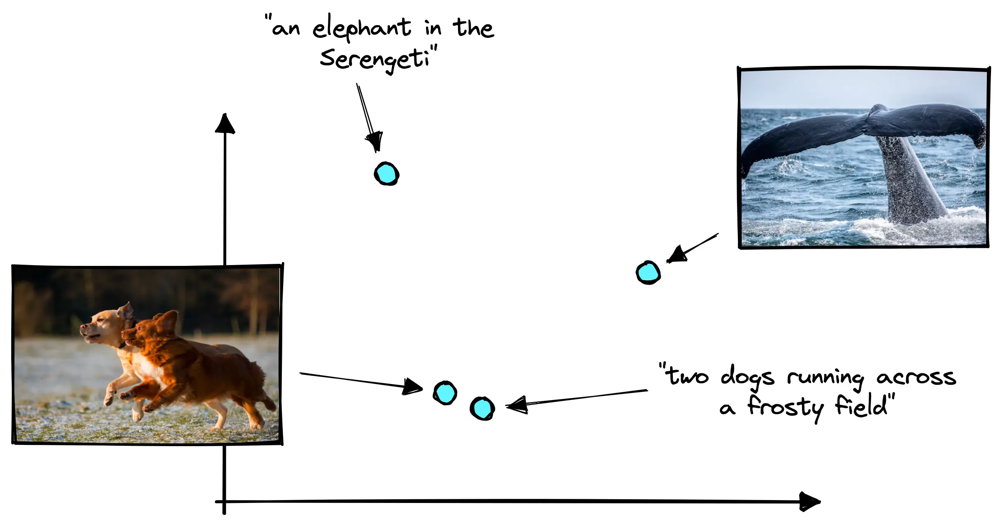
\includegraphics[width=0.7\textwidth]{archivos/clip_space.png}
  \caption[Espacio vectorial multimodal de CLIP]{Ejemplo conceptual de un espacio vectorial multimodal entrenado por \glsentryshort{clip}, donde imágenes y descripciones semánticas correspondientes se representan mediante vectores cercanos. (Fuente: \citep{noauthor_multi-modal_nodate}).}
  \label{fig:clip_space}
\end{figure}

\begin{figure}[h]
  \centering
  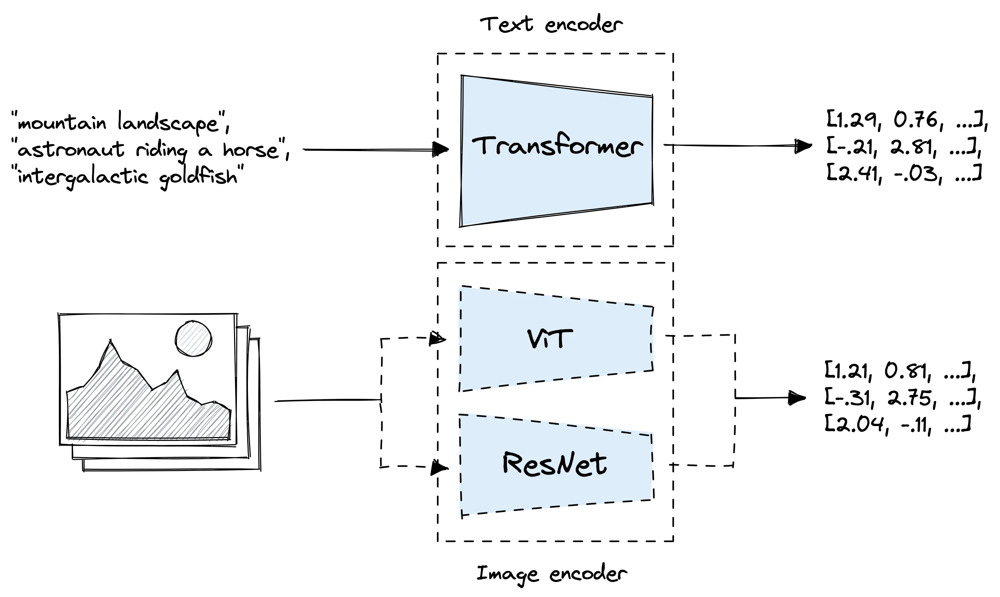
\includegraphics[width=0.7\textwidth]{archivos/clip_architecture.png}
  \caption[Arquitectura de CLIP]{Arquitectura del modelo \glsentryshort{clip}: encoder de texto y encoder de imagen que proyectan al mismo espacio de embedding. (Fuente: \citep{noauthor_multi-modal_nodate}).}
  \label{fig:clip_architecture}
\end{figure}

\subsection{Modelos Generativos de Descripción de Imágenes}

Otra campo de estudio importante se centra en los \textbf{modelos generativos de descripción de imágenes}. Estos sistemas realizan la tarea conocida como \emph{image captioning}, que consiste en generar una descripción en lenguaje natural para una imagen dada. Modelos recientes como \textbf{\gls{blip}-2} ejemplifican esta aproximación, combinando un encoder visual pre-entrenado, un modelo de lenguaje grande congelado y un transformador ligero intermedio denominado Q-Former. Esta arquitectura logra puentear eficientemente la brecha entre visión y lenguaje. El encoder de imagen extrae las características visuales relevantes, mientras que el \gls{llm} se encarga de generar la descripción textual coherente.

\subsection{VQA y Diálogo Multimodal}

Junto al desarrollo de modelos como \gls{blip}-2, han aparecido numerosos modelos abiertos que permiten la \textbf{\gls{vqa}} y el diálogo multimodal. Entre ellos destaca \textbf{\gls{llava}}, que utiliza GPT-4 para generar datos sintéticos de entrenamiento y posteriormente afina un modelo basado en \emph{Vicuna} (un derivado de LLaMA) acoplado a un encoder visual. Otro modelo relevante es \textbf{Moondream}, un \gls{vlm} open-source de tan solo 2 mil millones de parámetros (2B), capaz de operar en tiempo real incluso en CPUs o dispositivos móviles. Moondream ha demostrado capacidades notables en la generación de descripciones detalladas, la respuesta a preguntas visuales, la detección de objetos en modalidad cero-shot y el \gls{ocr} básico para leer texto en imágenes. En esta misma línea, \textbf{JoyCaption} se presenta como un modelo de captioning de imágenes libre y sin censura, concebido originalmente para generar descripciones ricas que ayuden a entrenar modelos de difusión. Finalmente, aunque de naturaleza propietaria, \textbf{GPT-4 con visión} (GPT-4V) ha demostrado capacidades impresionantes al responder con acierto a entradas que combinan imagen y texto, si bien su acceso limitado restringe su uso en entornos académicos.

En resumen, el estado del arte en la convergencia de imagen y lenguaje muestra de forma clara dos enfoques complementarios para la búsqueda multimedia. Por un lado, los \emph{embeddings} multimodales tipo \glsentryshort{clip} posibilitan una \textbf{búsqueda directa por similitud} entre consultas textuales y contenido visual. Por otro lado, los \emph{modelos generativos visiolingüísticos} facilitan la \textbf{descripción o comprensión de imágenes mediante texto}, lo que permite indexar y razonar sobre ellas utilizando lenguaje natural.

\section{Modelos Multimodales para Vídeo}

Extender la búsqueda basada en lenguaje natural al dominio del \textbf{vídeo} conlleva retos adicionales, pues los vídeos combinan secuencias de imágenes con audio y, en ocasiones, texto incrustado.

\subsection{Técnicas de Procesamiento de Video}

Para abordar la complejidad del procesamiento de vídeo, se emplean diversas técnicas. Una fundamental es el \textbf{análisis por frames}, que implica extraer fotogramas importantes o representativos del vídeo y aplicarles \glspl{vlm}, convirtiendo el problema de vídeo en el manejo de un conjunto de imágenes con marcas de tiempo. Por otro lado, el \textbf{procesamiento de audio} es crucial por lo que mediante modelos de \textbf{\gls{asr}} como \emph{Whisper}, es posible transcribir con alta calidad el diálogo o narración presente en los vídeos, permitiendo indexar cada vídeo por su transcripción textual completa. Además, se están desarrollando \textbf{modelos vídeo-texto end-to-end}, como \emph{VideoCLIP}, que extienden la idea de \glsentryshort{clip} al dominio temporal, o transformadores específicos para vídeo que realizan \emph{video captioning}.

\subsection{Arquitecturas para Búsqueda en Video}

Una arquitectura reciente para la búsqueda en vídeo combina los enfoques anteriores en un pipeline \gls{rag} multimodal. Este sistema indexa, por un lado, los \emph{frames} visuales mediante embeddings y, por otro, las transcripciones de voz como texto. Para una consulta, recupera fragmentos candidatos por similitud visual o textual, y posteriormente utiliza un modelo de lenguaje para sintetizar ambas fuentes de información y determinar la respuesta más adecuada.

\subsection{Modelos Unificados Multimodales}

Recientemente, han surgido modelos unificados que procesan múltiples modalidades de forma integrada. \textbf{MiniGPT-4}, por ejemplo, puede aceptar secuencias de imágenes como entrada, simulando un vídeo corto. \textbf{MiniCPM-V} soporta entradas de vídeo directamente, generando una descripción general del contenido. Google con \textbf{Gemini} ha avanzado en la integración de visión, vídeo y sonido en un mismo \gls{llm}, y Meta con \textbf{ImageBind} ha propuesto aprender una representación común para imágenes, texto, audio y otros sensores, abriendo nuevas vías para la comprensión multimodal holística.

\section{Análisis de Audio y Búsqueda mediante Sonido}

Para completar un buscador verdaderamente multimedia, es imprescindible considerar el contenido de \textbf{audio} independiente de los vídeos, como archivos de sonido o música.

\subsection{Procesamiento de Habla}

En el caso de que el audio contenga habla, como en podcasts, grabaciones o conferencias, se aplican técnicas de \gls{asr} con modelos robustos como Whisper. Esto permite obtener una transcripción textual que se convierte en contenido indexable, facilitando búsquedas por palabras clave o semántica mediante el uso de \glspl{llm} o embeddings textuales.

\subsection{Audio No Verbal}

Para el audio que no es voz, como sonidos ambientales, música o efectos sonoros, existen modelos como \textbf{\gls{clap}}. Este entrena conjuntamente un codificador de audio y uno de texto, lo que permite buscar efectos de sonido a partir de descripciones textuales (``sonido de lluvia'', ``pasos en la grava'') y facilita la clasificación cero-shot de audio.

\subsection{Modelos Generadores de Descripciones Auditivas}

Complementariamente, modelos como \textbf{AudioCaption} de Microsoft pueden generar frases descriptivas de clips de audio. Esta capacidad permite describir cada archivo de sonido en formato textual, indexar dichas descripciones y, en consecuencia, facilitar un acceso más semántico al contenido auditivo, más allá de simples metadatos.

\section{Comparativa de Modelos Representativos}
\label{sec:comparativa}

La tabla \ref{tab:comparativa_modelos} resume algunos modelos representativos, destacando la distinción entre modelos propietarios como ChatGPT y una creciente diversidad de iniciativas abiertas. Para el desarrollo de un sistema como \textbf{LLMSearch}, los módulos open-source son particularmente relevantes. Es factible combinar herramientas como MiniCPM-V, Moondream, Whisper y \gls{clap} para construir un sistema completo: Whisper se encargaría de la transcripción de audio; \gls{clap}, del indexado de sonidos no verbales; Moondream o \gls{blip}-2, de la descripción de imágenes; y un \gls{llm} generalista como Vicuna o LLaMA podría orquestar la interacción conversacional y la fusión de información.

\begin{table}[h!]
  \centering
  \captionsetup{justification=centering} % Centrar el texto del caption
  \resizebox{\textwidth}{!}{%
    \begin{tabular}{llll}
      \hline
      \textbf{Modelo} & \textbf{Modalidades} & \textbf{Tamaño} & \textbf{Características principales} \\ \hline
      ChatGPT (GPT-4)  & Texto (y visión en GPT-4V) & >100 B? & \glsentryshort{llm} propietario de OpenAI, rendimiento puntero en comprensión y generación de lenguaje. \\
      MiniCPM-V 2.5    & Texto, Imágenes, Vídeo, Audio & \textasciitilde8 B & Open-source, eficiente para despliegue en dispositivos; consultas multimodales. \\
      Moondream 2      & Imágenes–Texto & 2 B & \glsentryshort{vlm} ultraligero con \glsentryshort{vqa}, captioning, detección y \glsentryshort{ocr} en CPU en tiempo real. \\
      Whisper          & Audio–Texto & \textasciitilde1.6 B & \glsentryshort{asr} multilingüe de código abierto, muy robusto ante acentos y ruido. \\ \hline
    \end{tabular}%
  }
  \caption{Comparativa de modelos representativos en lenguaje y multimodalidad.}
  \label{tab:comparativa_modelos}
\end{table}

\section{Selección del Modelo Multimodal para Ejecución Local}

La elección de un modelo de lenguaje grande \gls{llm} con capacidades multimodales que pueda operar eficientemente en un entorno local es un componente crítico para el proyecto LLMSearch. Esta decisión impacta directamente en la viabilidad, el rendimiento y la accesibilidad del sistema para el usuario final. Para fundamentar esta elección, se ha realizado un análisis comparativo basado en métricas de rendimiento publicadas por plataformas especializadas, como se observa en la Figura~\ref{fig:tabla_comparativa_modelos} y las visualizaciones gráficas de la Figura~\ref{fig:graficas_rendimiento_modelos}.

\begin{figure}[H]
  \centering
  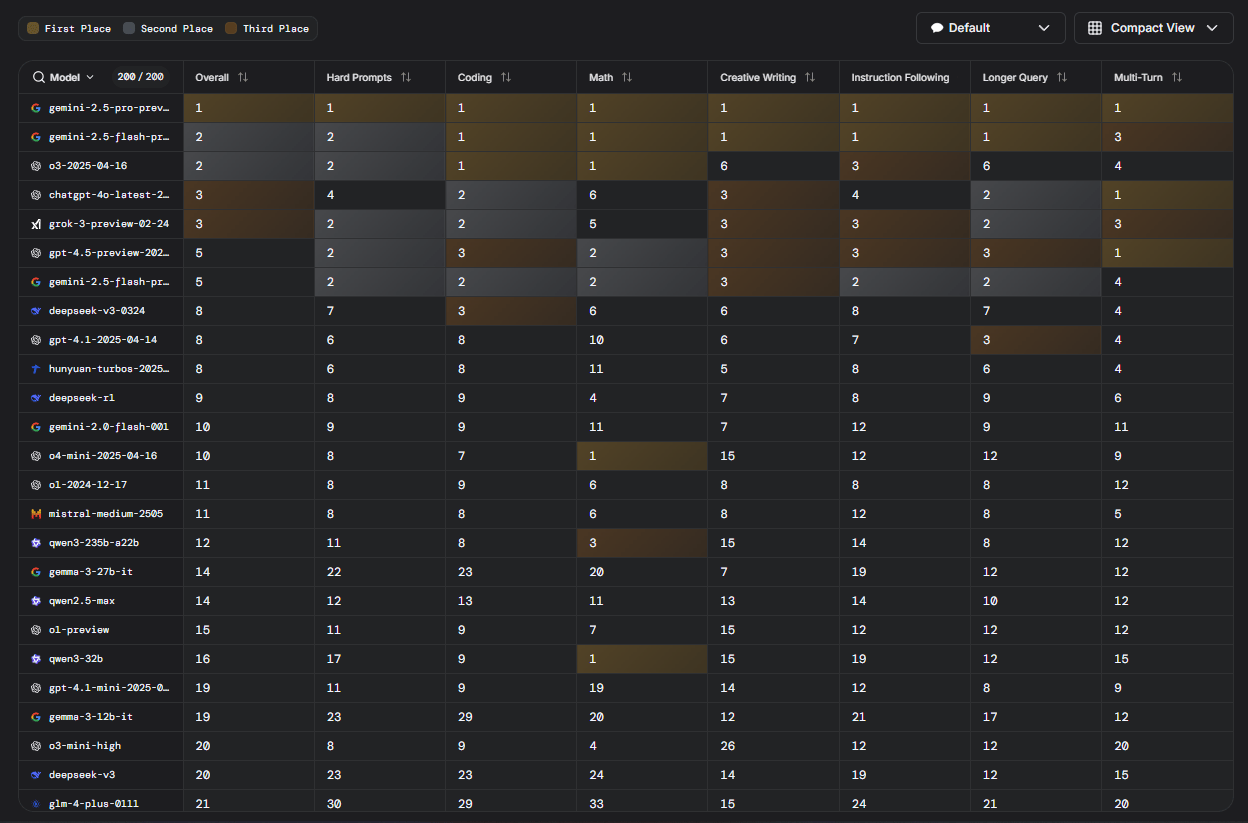
\includegraphics[width=\textwidth]{archivos/tabla_comparativa_modelos.png}
  \caption{Tabla comparativa de rendimiento de diversos modelos LLM en diferentes benchmarks (Fuente: \citep{noauthor_lmarena_nodate}).}
  \label{fig:tabla_comparativa_modelos}
\end{figure}

\begin{figure}[H]
  \centering
  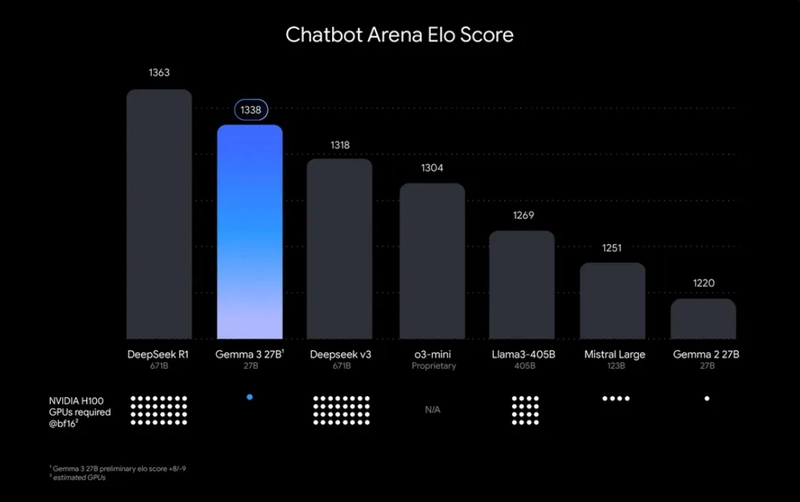
\includegraphics[width=\textwidth]{archivos/elo_score_gemma_vs_deepseek.png}
  \caption{Gráfico comparativo de rendimiento de modelos en el benchmark ELO junto al número de GPUs requeridas para su ejecución. (Fuente: \citep{noauthor_gemma_nodate}).}
  \label{fig:graficas_rendimiento_modelos}
\end{figure}

El principal requisito para LLMSearch es la capacidad de procesar información multimodal (texto e imágenes) y ejecutar todas las operaciones de inferencia en la máquina local del usuario, utilizando herramientas como LMStudio que facilitan la gestión de modelos abiertos. Esto implica descartar modelos propietarios que requieren acceso a API externas (e.g., modelos de OpenAI, Google Cloud) o aquellos con un número de parámetros excesivamente grande (e.g., superiores a $\approx$30B) que harían inviable su ejecución en hardware de consumo estándar, incluso con técnicas de cuantización.

Considerando estos factores, y analizando los datos presentados, los siguientes modelos emergen como candidatos viables:

\begin{itemize}
  \item \textbf{Gemma (familia de modelos de Google):} Estos modelos, como \texttt{gemma-3-12b-it} o \texttt{gemma-3-27b-it} \citep{noauthor_welcome_2025}, son inherentemente multimodales y están diseñados para ser eficientes y abiertos. El proyecto ya contempla el uso de Gemma para el análisis multimodal, lo que facilitaría la coherencia y la integración. La variante de 12 mil millones de parámetros (12B) representa un compromiso interesante entre capacidad y requisitos computacionales para un entorno local.
  \item \textbf{Mistral (familia de modelos de Mistral AI):} Modelos como \texttt{mistral-medium-2505} son reconocidos por su excelente rendimiento en tareas textuales y su eficiencia. Sin embargo, para una funcionalidad multimodal integrada en un único modelo, se requeriría una variante específica o la combinación con un modelo de visión dedicado, lo cual podría añadir complejidad si se busca una solución unificada.
  \item \textbf{Modelos Gemini Flash (Google):} Versiones más ligeras como \texttt{gemini-2.0-flash-001} son también multimodales por diseño. No obstante, su disponibilidad y madurez para ejecución puramente local a través de herramientas como LMStudio podría ser un factor a considerar en comparación con Gemma o Mistral, que cuentan con un ecosistema GGUF muy consolidado.
\end{itemize}

\section{Conclusión}
\label{sec:conclusion}

Estudiado el estado del arte, se ha identificado la necesidad de construir un sistema que integre las capacidades de búsqueda y recuperación de información en múltiples modalidades, como texto, imagen y audio. La combinación de \glspl{llm} con modelos visiolingüísticos y de audio permitirá abordar la búsqueda multimedia de manera más efectiva, facilitando la interacción del usuario mediante lenguaje natural.